% \subsection{Motivation}

\begin{frame}{Multi-Spectral Imaging}
  \begin{itemize}
    \item Multiple channels, small bandwidths.
    \item Enables spectral un-mixing.
    \item Our focus: thermal spectrum, between $7-14 \mu m$ (geospatial analysis). 
    \item Issues: expensive, no multispectral thermal data.
  \end{itemize}

  \begin{figure}
    \centering
    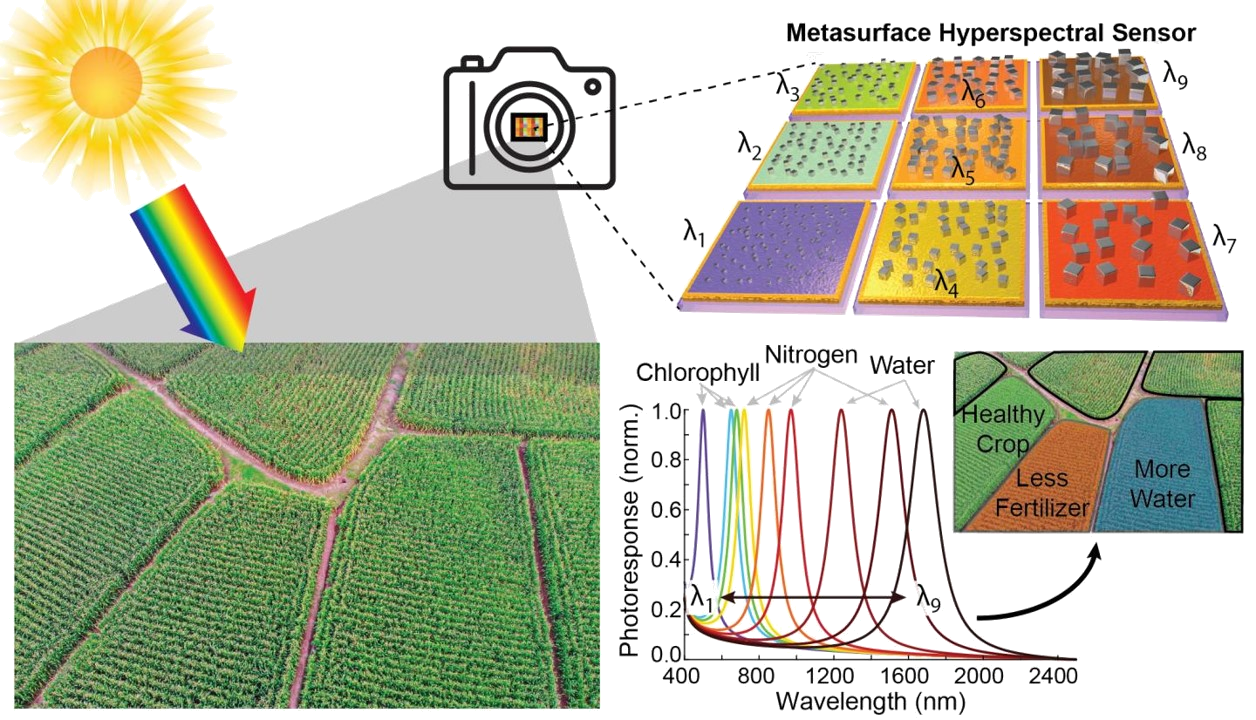
\includegraphics[width=0.5\linewidth]{../figs/introduction/multispectral.png}
  \end{figure}  
\end{frame}

\begin{frame}{Data Collection}
  \begin{itemize}
        \item Lightweight airplane.
        \item Simple thermal camera (FLIR TAU2), several flights, each with some IR filter (monochromatic) or without (panchromatic).
        \item Registration issue. Solution: unpaired image-to-image (UI2I) translation models.
    \end{itemize}
    \begin{figure}
        \centering
        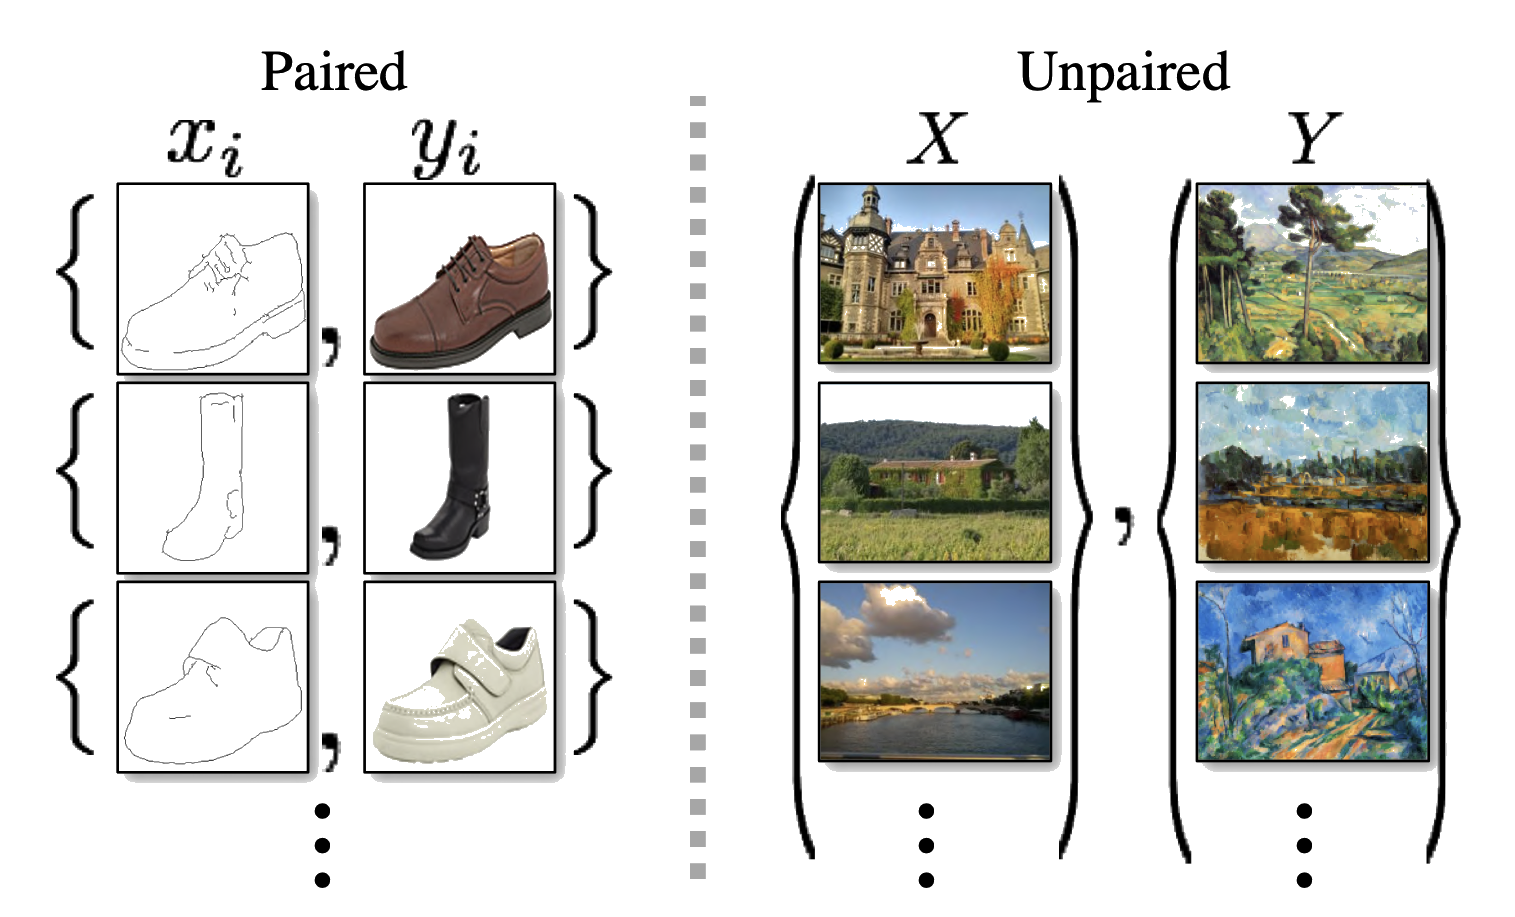
\includegraphics[width=0.5\linewidth]{../figs/related_work/paird_vs_unpaired_I2I.png}
      \end{figure}
  \end{frame}

\begin{frame}{Research Motivation}
  \vspace{-0.5cm}
  \begin{exampleblock}{Goal}
    Learn an UI2I transformation between different thermal spectra.
  \end{exampleblock} 
  \begin{exampleblock}{Hypothesis}
    Unique thermal physics can improve the quality of deep UI2I models.
  \end{exampleblock}  
  \begin{exampleblock}{Showcase}
    Transformation of wide-band (panchromatic) thermal images and to narrow-band (monochromatic) thermal images.
  \end{exampleblock}
\end{frame}